\documentclass[a4paper,12pt]{article}
%%%%%%%%%%%%%%%%%%%%%%%%%%%%%%%%%%%%%%%%%%%%%%%%%%%%%%%%%%%%%%%%%%%%%%%%%%%%%%%%%%%%%%%%%%%%%%%%%%%%%%%%%%%%%%%%%%%%%%%%%%%%%%%%%%%%%%%%%%%%%%%%%%%%%%%%%%%%%%%%%%%%%%%%%%%%%%%%%%%%%%%%%%%%%%%%%%%%%%%%%%%%%%%%%%%%%%%%%%%%%%%%%%%%%%%%%%%%%%%%%%%%%%%%%%%%
\usepackage{eurosym}
\usepackage{vmargin}
\usepackage{amsmath}
\usepackage{graphics}
\usepackage{epsfig}
\usepackage{framed}
\usepackage{subfigure}
\usepackage{fancyhdr}

\setcounter{MaxMatrixCols}{10}
%TCIDATA{OutputFilter=LATEX.DLL}
%TCIDATA{Version=5.00.0.2570}
%TCIDATA{<META NAME="SaveForMode"CONTENT="1">}
%TCIDATA{LastRevised=Wednesday, February 23, 201113:24:34}
%TCIDATA{<META NAME="GraphicsSave" CONTENT="32">}
%TCIDATA{Language=American English}

\pagestyle{fancy}
\setmarginsrb{20mm}{0mm}{20mm}{25mm}{12mm}{11mm}{0mm}{11mm}
\lhead{Advanced Data Modelling} \rhead{Logistic Regression} \chead{MA4128} %\input{tcilatex}

%---------------------------------------------------------%
\begin{document}

\section{Model Diagnostics for Logistic Regression}
%http://statistics.ats.ucla.edu/stat/mult_pkg/faq/general/Psuedo_RSquareds.htm

%http://www.strath.ac.uk/aer/materials/5furtherquantitativeresearchdesignandanalysis/unit6/goodnessoffitmeasures/

\subsection{Omnibus Test for Model Coefficients}
The overall significance is tested using what SPSS calls the \textbf{\textit{Model Chi-square}}, which is derived from the likelihood of observing the actual data under the assumption that the model that has been fitted is accurate. There are two hypotheses to test in relation to the overall fit of the model:

\begin{framed}
\begin{itemize}
	\item[$H_0$] The model is a good fitting model.
	\item[$H_1$] The model is not a good fitting model (i.e. the predictors have a significant effect).
\end{itemize}
\end{framed}

\begin{itemize}
	\item For the example provided here, the model chi square has 2 degrees of freedom, a value of 24.096 and a probability of $p < 0.000$. \textit{(see Next Page for SPSS Output)}.
	
	\item Thus, the indication is that the model has a poor fit, with the model containing only the constant indicating that the predictors do have a significant effect and create essentially a different model. 
	\item So we need to look closely at
	the predictors and from later tables determine if one or both are significant predictors.
\end{itemize}
\bigskip

\noindent \textbf{Remark upon ``Steps"}
\begin{itemize}
	\item This table has 1 step. This is because we are entering both variables and at the same
	time providing only one model to compare with the constant model. 
	\item In stepwise logistic regression there are a number of steps listed in the table as each variable is added or
	removed, creating different models. 
	\item The step is a measure of the improvement in the
	predictive power of the model since the previous step. 
	\item I will revert to this next class.
\end{itemize}

\subsection{Model Summary Table}

\begin{itemize}
	\item The likelihood function can be thought of as a measure of how well a candidate model fits the data (although that is a very simplistic definition). 
	\item Later on in the course, we will meet the AIC Function. The AIC criterion is based on the Likelihood function.
	\item The likelihood function of a fitted model is commonly re-expressed as $-2LL$ (i.e. The log of the likelihood times minus 2). The –2LL value from the Model Summary table below is 17.359.
	\item It is not immediately clear how to interpret $-2LL$ yet. However this measure is useful in comparing various candidate models, and is therefore used in \textbf{\textit{Variable Selection Procedure}}, such as backward and forward selection.
\end{itemize}

\begin{figure}[h!]
\centering
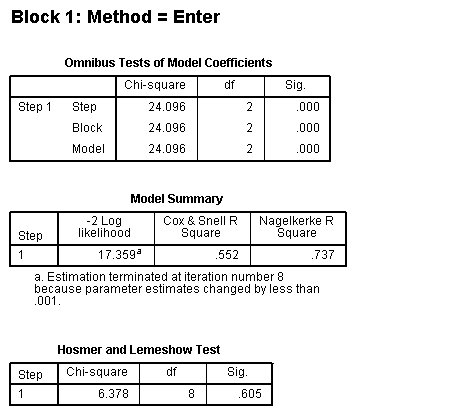
\includegraphics[width=0.9\linewidth]{images/Logistic5}
\end{figure}





%---------------------------------------------------------- %
\newpage






\subsection{Hosmer-Lemeshow Goodness-of-Fit Test}
\begin{framed}
\begin{itemize}
	\item The Hosmer-Lemeshow Goodness-of-Fit
	test tells us whether we have constructed a valid overall model or not, and is an alternative to model chi square procedure.
	\item If the model is a good fit to the data then the Hosmer-Lemeshow Goodness-of-Fit test should have an associated p-value greater than 0.05.
\end{itemize} 
\end{framed}
If the H-L goodness-of-fit test statistic is greater than .05, as we want for well-fitting models, we fail to reject the null hypothesis that there is no difference between observed and model-predicted values, implying that the model’s estimates fit the data at an acceptable level. That is, well-fitting models show non-significance on the
H-L goodness-of-fit test. This desirable outcome of non-significance indicates that the
model prediction does not significantly differ from the observed.

\noindent \textbf{Performing the Hosmer-Lemeshow Goodness-of-Fit Test} 	
\begin{itemize}	
\item 	
	The Hosmer-Lemeshow test of goodness of fit is not automatically a part of the SPSS logistic regression output. 
	To get this output, we need to go into \textbf{\texttt{options}} and tick the box marked Hosmer-Lemeshow test of goodness of fit. 
\end{itemize}



In our example, this gives us the following output:

\begin{center}
	\begin{tabular}{|c|c|c|c|}
		\hline  Step	& Chi-square&	df 	 & Sig. \\ \hline
		1	 & 142.032	& 6	 &.000 \\ 
		\hline 
	\end{tabular} 
\end{center}


Therefore, our model is significant, suggesting it does not fit the data. However, as we have a sample size of over 13,000, even very small divergencies of the model from the data would be flagged up and cause significance. Therefore, with samples of this size it is hard to find models that are parsimonious (i.e. that use the minimum amount of independent variables to explain the dependent variable) and fit the data. Therefore, other fit indices might be more appropriate.\\

% Binary Regression : http://teaching.sociology.ul.ie/SSS/lugano/node10.html 
% http://istics.net/pdfs/multivariate.pdf
%---------------------------------------------------------- %

\noindent \textbf{Computing the Hosmer and Lemeshow Test Statistic}

\begin{itemize}
	\item The Hosmer and Lemeshow test
	divides subjects into 10 ordered groups of subjects and then compares the number
	actually in the each group (observed) to the number predicted by the logistic regression
	model (predicted). 
	\item The 10 ordered groups are created based on their estimated probability; those with estimated probability below .1 form one group, and so on, up to those with probability .9 to 1.0.
	\item 
	Each of these categories is further divided into two groups based on the actual observed outcome variable (success, failure). The expected frequencies for each of the cells are obtained from the model. A probability (p) value is
	computed from the chi-square distribution with 8 degrees of freedom to test the fit of the logistic model.
	
\end{itemize}
\begin{figure}[h!]
	\begin{center}
		% Requires \usepackage{graphicx}
		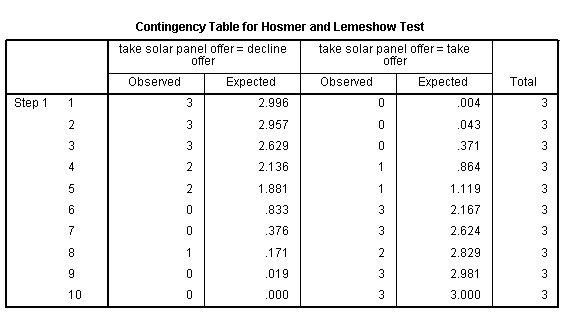
\includegraphics[scale=0.6]{images/Logistic6}\\
		\caption{Hosmer and Lemeshow Table}
	\end{center}
\end{figure}

\noindent \textbf{Sample Adequacy}\\


The H-L statistic assumes sampling adequacy, with a rule of thumb being enough cases so that 95\% of cells (typically, 10 decile groups times 2 outcome categories = 20 cells) have an expected frequency $>$ 5. Our H-L statistic has a significance of .605 which means that it is not statistically significant and therefore our model is quite a
good fit.
\begin{figure}[h!]
	\begin{center}
		% Requires \usepackage{graphicx}
		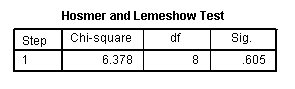
\includegraphics[scale=0.6]{images/Logistic7A}\\
		\caption{Hosmer and Lemeshow Statistic}
	\end{center}
\end{figure}

\section{R Squared Diagnostics}
\begin{itemize}
	\item In order to understand how much variation in the dependent variable can be explained by the model (the equivalent of $R^2$ in multiple regression), you should consult \textbf{\textit{Model Summary}} statistics.
	
	\item 
	Logistic regression does not have an equivalent to the R-squared that is found in OLS regression; however, many researchers have tried to come up with one. 
	
	
	\item The SPSS output table below contains the \textit{Cox \& Snell R Square} and \textit{Nagelkerke R Square }values, which are both methods of calculating the explained variation. These values are sometimes referred to as pseudo $R^2$ values (and will have lower values than in multiple regression).
	\item  However, they are interpreted in the same manner, but with more caution. Therefore, the explained variation in the dependent variable based on our model ranges from 24.0\% to 33.0\%, depending on whether you reference the Cox \& Snell $R^2$ or Nagelkerke $R^2$ methods, respectively. 
	
	\item Nagelkerke $R^2$ is a modification of Cox \& Snell $R^2$, the latter of which cannot achieve a value of 1. For this reason, it is preferable to report the Nagelkerke $R^2$ value.
\end{itemize}

\begin{figure}[h!]
	\centering
	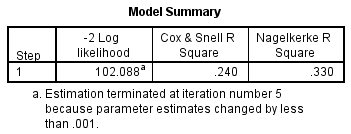
\includegraphics[width=0.9\linewidth]{images/BLogReg-Rsq}
	\caption{SPSS output}
	\label{fig:BLogReg-Rsq}
\end{figure}
\begin{itemize}
\item Although there is no close analogous statistic in logistic regression to
the coefficient of determination $R^2$ the Model Summary Table provides some approximations. Cox and Snell’s R-Square attempts to imitate multiple R-Square based on ‘likelihood’, but its maximum can be (and usually is) less than 1.0, making it difficult to interpret. 
\item Here it is indicating that 55.2\% of the variation in the DV is explained by the
logistic model. 
\item Logistic regression does not have an equivalent to the R-squared that is found in OLS regression; however, many people have tried to come up with one.  
Cox  and Snell R Square and Nagelkerke R Square - These are pseudo R-squares. 
\item 	Nagelkerke's R-Square is a further modification of the Cox and Snell coefficient to assure that it can vary from 0 to 1. Nagelkerke's R-Square will normally be higher than the Cox and Snell measure. It is part of SPSS output and is the most-reported of the R-squared estimates.

\item The Nagelkerke modification that does range from 0 to 1 is a more reliable
measure of the relationship. Nagelkerke’s $R^2$ will normally be higher than the Cox and Snell measure.



\item \textbf{Cox and Snell's R-Square} is an attempt to imitate the interpretation of multiple R-Square based on the likelihood, but its maximum can be (and usually is) less than 1.0, making it difficult to interpret. It is part of SPSS output.
\end{itemize}
%==============================================================%

\subsubsection{Nagelkerke's R-Square}
\begin{itemize}
	\item  Nagelkerke’s $R^2$ is part of SPSS output in the ‘Model Summary’ table and is the most-reported of the R-squared estimates. 
	\item In our case it is 0.737, indicating a moderately strong relationship of 73.7\% between the predictors and the prediction.
	
	

\end{itemize}




\subsection{Pseudo R-squares}
Cox \& Snell R Square and Nagelkerke R Square are two measures from the \textbf{pseudo R-squares} family of measures.


There are a wide variety of pseudo-R-square statistics (these are only two of them).  Because this statistic does not mean what R-squared means in OLS regression (the proportion of variance explained by the predictors), we suggest interpreting this statistic with great caution.


\section{Likelihood Ratio Test}
\begin{itemize}
	\item The likelihood ratio test is a test of the difference between -2LL for the full
	model with predictors and ?2LL for initial chi-square in the null model.
	\item When probability fails to reach the 5\% significance level, we retain the null hypothesis
	that knowing the independent variables (predictors) has no increased effects (i.e. make no
	difference) in predicting the dependent.
\end{itemize}



\end{document}